\documentclass[12pt,a4paper]{article}

% NOTE FOR OVERLEAF: If the .tex file is placed at project root (not inside reports/),
% change all "../outputs/" paths to "outputs/" using find-and-replace.
% Also: heatmap filenames contain spaces and parentheses. If grffile doesn't help,
% rename the uploaded files to remove spaces (e.g., FAKE_48_5.jpg).

% ── Packages ──
\usepackage[margin=2.5cm]{geometry}
\usepackage{graphicx}
\usepackage{booktabs}
\usepackage{hyperref}
\usepackage{amsmath}
\usepackage{xcolor}
\usepackage{float}
\usepackage{caption}
\usepackage{subcaption}
\usepackage{enumitem}
\usepackage{fancyhdr}
\usepackage{titlesec}
\usepackage{grffile}
% If you later create a .bib file, uncomment these:
% \usepackage[backend=biber,style=ieee]{biblatex}
% \addbibresource{references.bib}

\hypersetup{
    colorlinks=true,
    linkcolor=blue!70!black,
    citecolor=blue!70!black,
    urlcolor=blue!70!black,
}

% ── Header/Footer ──
\pagestyle{fancy}
\fancyhf{}
\fancyhead[L]{\small AI-Generated Image Detection}
\fancyhead[R]{\small Progress Report}
\fancyfoot[C]{\thepage}
\renewcommand{\headrulewidth}{0.4pt}

% ── Section formatting ──
\titleformat{\section}{\large\bfseries}{}{0em}{}[\titlerule]
\titleformat{\subsection}{\normalsize\bfseries}{}{0em}{}

% ══════════════════════════════════════════════════════════════
\begin{document}

% ── Title Page ──
\begin{titlepage}
\centering
\vspace*{3cm}
{\Huge\bfseries Progress Report\par}
\vspace{1cm}
{\LARGE AI-Generated Image Detection\par}
\vspace{0.5cm}
{\large\itshape Evaluating Generalisation Across Generative Model Generations\par}
\vspace{3cm}

\begin{tabular}{rl}
\textbf{Author:}      & Krishi Rajeshkumar Shah (220968905) \\
\textbf{Supervisor:}   & Mona Nasery \\
\textbf{Course:}       & EECS 4080 --- Computer Science Project \\
\textbf{Date:}         & June 2026 \\
\end{tabular}

\vfill
\end{titlepage}

\tableofcontents
\newpage

% ══════════════════════════════════════════════════════════════
\section{Introduction and Motivation}

AI-generated images have become increasingly difficult to distinguish from authentic photographs. While detection tools exist, they are predominantly trained and evaluated on datasets of images generated by older generative models. As newer architectures such as Stable Diffusion~3, Midjourney~v6, and GPT-4o produce increasingly realistic outputs, a critical question emerges: \textbf{do existing detectors still work, and if not, why?}

This project investigates the \emph{generalisation gap} in AI-generated image detection --- the degree to which a detector trained on one generation of synthetic images degrades when tested against images produced by newer, more capable models. The hypothesis is that current detectors rely on low-level statistical artefacts specific to the architectures they were trained on, and that these artefacts are no longer reliably present in outputs from state-of-the-art generative models.

\medskip
\noindent\textbf{Research Question:} \emph{How well do AI-generated image detectors trained on current benchmark datasets generalise to images produced by next-generation generative models, and what accounts for the performance gap?}

% ══════════════════════════════════════════════════════════════
\section{Brief Literature Review}

\textbf{Wang et al.\ (2020)} trained a ResNet-50 on ProGAN images and showed it generalised surprisingly well across 11 other GAN architectures, primarily because data augmentation (blur, JPEG compression) forced the model to learn shared GAN fingerprints. However, this study predates diffusion models entirely.

\textbf{Bird and Lotfi (2024)} created the CIFAKE dataset (60K images) and demonstrated $>$92\% detection accuracy using standard architectures. They used LIME for explainability; this project replaces it with Grad-CAM for faster, more spatially coherent heatmaps.

\textbf{Corvi et al.\ (2023)} showed a clear generalisation gap: GAN-trained classifiers dropped to near-chance accuracy (50--60\%) on diffusion model outputs and vice versa. Their frequency analysis showed GAN and diffusion images occupy separate regions in feature space.

\textbf{Gragnaniello et al.\ (2021)} demonstrated that different GANs leave different fingerprints and that there is a trade-off between in-distribution accuracy and cross-generator transferability.

\textbf{Guo et al.\ (2017)} established that modern deep networks are poorly calibrated and proposed temperature scaling as a simple, effective post-hoc calibration method.

\textbf{Selvaraju et al.\ (2017)} introduced Grad-CAM for visual explanations of CNN decisions via gradient-weighted class activation mapping.

\medskip
\noindent\textbf{Research Gap:} No existing study combines (1) testing across four chronologically distinct generator families, (2) measuring calibration alongside accuracy, (3) using Grad-CAM comparatively across generator families, and (4) focusing on measuring the generalisation problem rather than proposing a new detector.

% ══════════════════════════════════════════════════════════════
\section{Dataset Description: CIFAKE}

The primary training and evaluation dataset is \textbf{CIFAKE} (Bird \& Lotfi, 2024), downloaded from Kaggle. Table~\ref{tab:dataset} summarises its properties.

\begin{table}[H]
\centering
\caption{CIFAKE dataset properties.}
\label{tab:dataset}
\begin{tabular}{ll}
\toprule
\textbf{Property} & \textbf{Detail} \\
\midrule
Total images       & 60,000 (balanced) \\
Real images        & 30,000 (sourced from CIFAR-10) \\
AI-generated       & 30,000 (Stable Diffusion v1.4) \\
Resolution         & $32 \times 32$ pixels (upscaled to $224 \times 224$) \\
Format             & RGB (3 channels) \\
Classes            & FAKE (class 0), REAL (class 1) \\
\bottomrule
\end{tabular}
\end{table}

The train/validation split is created by randomly splitting the CIFAKE training folder 80/20 with a fixed seed (42) for reproducibility. The test set is the separate CIFAKE test folder. All three splits are balanced at approximately 50\% FAKE / 50\% REAL, as shown in Table~\ref{tab:splits}.

\begin{table}[H]
\centering
\caption{Dataset splits (verified balanced).}
\label{tab:splits}
\begin{tabular}{lrrrl}
\toprule
\textbf{Split} & \textbf{FAKE (0)} & \textbf{REAL (1)} & \textbf{Total} & \textbf{\% FAKE} \\
\midrule
Train      & 39,962 & 40,038 & 80,000 & 50.0\% \\
Validation & 10,038 &  9,962 & 20,000 & 50.2\% \\
Test       & 10,000 & 10,000 & 20,000 & 50.0\% \\
\bottomrule
\end{tabular}
\end{table}

Both REAL and FAKE images use the identical preprocessing pipeline --- they are loaded together via PyTorch's \texttt{ImageFolder}, which applies the same transforms to all images regardless of class.

% ══════════════════════════════════════════════════════════════
\section{Methodology and Model Architecture}

\subsection{Architecture}

The detector is an \textbf{EfficientNet-B3} pretrained on ImageNet, loaded via the \texttt{timm} library. The original classifier head is replaced with a linear layer mapping the 1,536-dimensional feature vector to 2 output classes:

\begin{verbatim}
EfficientNet-B3 (ImageNet pretrained)
  └── classifier: Linear(1536, 2)
\end{verbatim}

This is a binary classification model outputting logits for [FAKE, REAL], converted to probabilities via softmax.

\subsection{Label Mapping}

PyTorch's \texttt{ImageFolder} sorts class folders alphabetically, producing:
\begin{itemize}[noitemsep]
    \item \textbf{FAKE = class 0} (folder name: \texttt{FAKE})
    \item \textbf{REAL = class 1} (folder name: \texttt{REAL})
\end{itemize}
This mapping is consistent across all splits. The model's softmax output at index~0 gives $P(\text{FAKE})$ and at index~1 gives $P(\text{REAL})$. A sample is classified as FAKE if $P(\text{FAKE}) > 0.5$ (default threshold).

\subsection{Post-hoc Calibration}

After training, confidence calibration is applied using \textbf{temperature scaling} (Guo et al., 2017). A single scalar parameter $T$ is \emph{learned} (not set manually) on the validation set by minimising negative log-likelihood using L-BFGS optimisation:
\[
    \text{calibrated\_probs} = \text{softmax}(\text{logits} / T)
\]
The temperature is initialised at 1.5 and optimised for up to 50 L-BFGS iterations. The learned value was $T = 1.2189$, indicating the model was slightly overconfident ($T > 1$ softens the distribution).

\subsection{Visual Explainability}

\textbf{Grad-CAM} (Selvaraju et al., 2017) is integrated using the \texttt{pytorch-grad-cam} library. The target layer is the last convolutional block of EfficientNet-B3 (\texttt{model.blocks[-1]}), which provides the highest-level spatial features before the classifier head.

% ══════════════════════════════════════════════════════════════
\section{Training Setup and Preprocessing}

\subsection{Hyperparameters}

A hyperparameter sweep over 6 combinations (2 learning rates $\times$ 3 weight decays) was run for 3 epochs each. The best combination was selected based on validation accuracy and used for the full 20-epoch training run. Table~\ref{tab:hyperparams} lists the configuration.

\begin{table}[H]
\centering
\caption{Training hyperparameters.}
\label{tab:hyperparams}
\begin{tabular}{ll}
\toprule
\textbf{Parameter} & \textbf{Value} \\
\midrule
Epochs (sweep)      & 3 per combination \\
Epochs (full)       & 20 \\
Learning rate       & Selected from sweep: \{1e-4, 3e-4\} \\
Weight decay        & Selected from sweep: \{1e-4, 1e-5, 1e-6\} \\
Batch size          & 32 \\
Optimiser           & AdamW \\
Scheduler           & CosineAnnealingLR ($T_{\max} = 20$) \\
Loss function       & CrossEntropyLoss \\
Random seed         & 42 \\
\bottomrule
\end{tabular}
\end{table}

\subsection{Train/Validation/Test Split}

The CIFAKE training set (60,000 images) is split 80/20 into train and validation sets using a fixed random seed (42) for reproducibility. The CIFAKE test folder (20,000 images) is used as the held-out test set. The resulting split:
\begin{itemize}[noitemsep]
    \item \textbf{Train:} 80,000 images (39,962 FAKE, 40,038 REAL)
    \item \textbf{Validation:} 20,000 images (10,038 FAKE, 9,962 REAL)
    \item \textbf{Test:} 20,000 images (10,000 FAKE, 10,000 REAL)
\end{itemize}
All splits are balanced at approximately 50\% FAKE / 50\% REAL, verified in Section~\ref{sec:balance}.

\subsection{Preprocessing}

\textbf{Training transforms} (applied identically to both FAKE and REAL):
\begin{enumerate}[noitemsep]
    \item \texttt{Resize(224)} --- scale to model input size
    \item \texttt{RandomHorizontalFlip()} --- augmentation
    \item \texttt{RandomCrop(224, padding=8)} --- augmentation
    \item \texttt{ColorJitter(0.2, 0.2, 0.2, 0.1)} --- augmentation
    \item \texttt{ToTensor()} --- convert to $[0, 1]$ float tensor
    \item \texttt{Normalize(mean=[0.485, 0.456, 0.406], std=[0.229, 0.224, 0.225])} --- ImageNet normalisation
\end{enumerate}

\textbf{Validation and test transforms} (applied identically to both FAKE and REAL):
\begin{enumerate}[noitemsep]
    \item \texttt{Resize(256)}
    \item \texttt{CenterCrop(224)}
    \item \texttt{ToTensor()}
    \item \texttt{Normalize(mean=[0.485, 0.456, 0.406], std=[0.229, 0.224, 0.225])}
\end{enumerate}

\subsection{Verification: Identical Preprocessing for Both Classes}

Both REAL and FAKE images are loaded via a single \texttt{ImageFolder} call, which assigns the same transform pipeline to every image regardless of its class label. There is no class-conditional preprocessing --- both classes undergo identical resizing, augmentation, tensor conversion, and normalisation. This was explicitly verified by inspecting the data loader code and confirming that the \texttt{transform} argument is shared.

% ══════════════════════════════════════════════════════════════
\section{Experimental Results}

\subsection{Overall Performance}

The trained checkpoint (epoch 2, validation accuracy 0.9694) was evaluated on the 20,000-image CIFAKE test set. Results are summarised in Table~\ref{tab:overall}.

\begin{table}[H]
\centering
\caption{Overall test-set performance.}
\label{tab:overall}
\begin{tabular}{lr}
\toprule
\textbf{Metric} & \textbf{Value} \\
\midrule
Test Accuracy                        & \textbf{96.96\%} \\
AUC-ROC                             & \textbf{0.9971} \\
ECE (before calibration, test set)   & 0.0026 \\
ECE (after calibration, test set)    & 0.0113 \\
Learned Temperature                  & 1.2189 \\
\bottomrule
\end{tabular}
\end{table}

\subsection{Per-Class Performance}

Both classes achieve similar precision, recall, and F1 --- there is no systematic imbalance (Table~\ref{tab:perclass}).

\begin{table}[H]
\centering
\caption{Per-class classification report on CIFAKE test set.}
\label{tab:perclass}
\begin{tabular}{lcccc}
\toprule
\textbf{Class} & \textbf{Precision} & \textbf{Recall} & \textbf{F1-Score} & \textbf{Support} \\
\midrule
FAKE (class 0) & 0.9858 & 0.9529 & 0.9691 & 10,000 \\
REAL (class 1) & 0.9544 & 0.9863 & 0.9701 & 10,000 \\
\midrule
Accuracy       &        &        & 0.9696 & 20,000 \\
Macro avg      & 0.9701 & 0.9696 & 0.9696 & 20,000 \\
\bottomrule
\end{tabular}
\end{table}

\subsection{Confusion Matrix}

\begin{table}[H]
\centering
\caption{Confusion matrix on CIFAKE test set.}
\label{tab:confusion}
\begin{tabular}{lcc}
\toprule
 & \textbf{Predicted FAKE} & \textbf{Predicted REAL} \\
\midrule
\textbf{Actual FAKE} & 9,529 (TP) & 471 (FN) \\
\textbf{Actual REAL} & 137 (FP)   & 9,863 (TN) \\
\bottomrule
\end{tabular}
\end{table}

\begin{figure}[H]
\centering
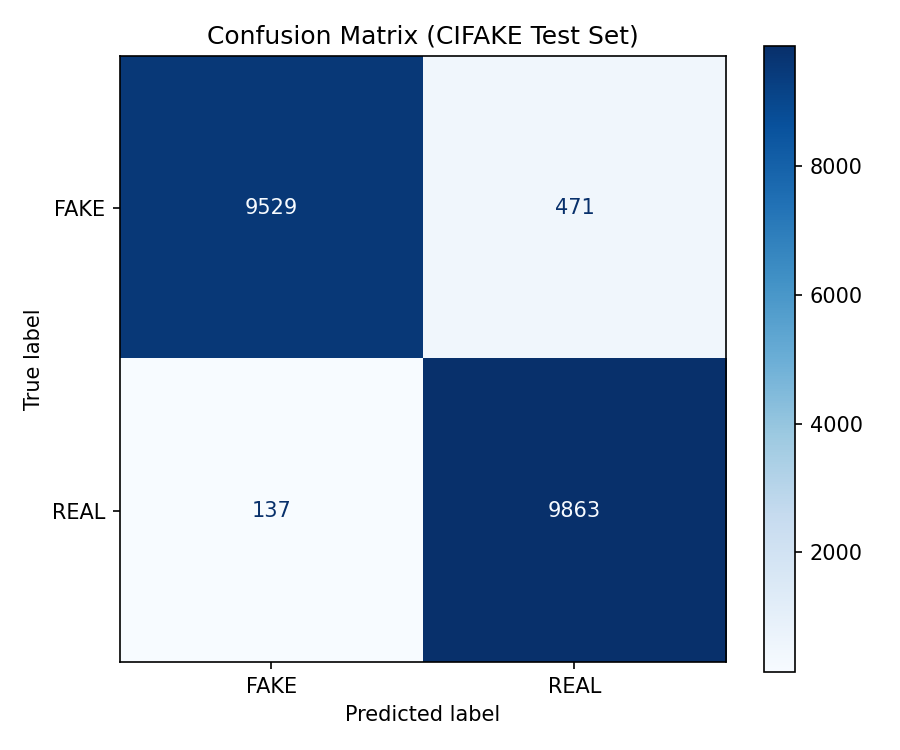
\includegraphics[width=0.7\textwidth]{../outputs/plots/confusion_matrix.png}
\caption{Confusion matrix on CIFAKE test set (20,000 images).}
\label{fig:confusion}
\end{figure}

\subsection{ROC Curve}

The ROC curve (Figure~\ref{fig:roc}) shows near-perfect discrimination with AUC-ROC = 0.9971, confirming the model performs well across all possible decision thresholds.

\begin{figure}[H]
\centering
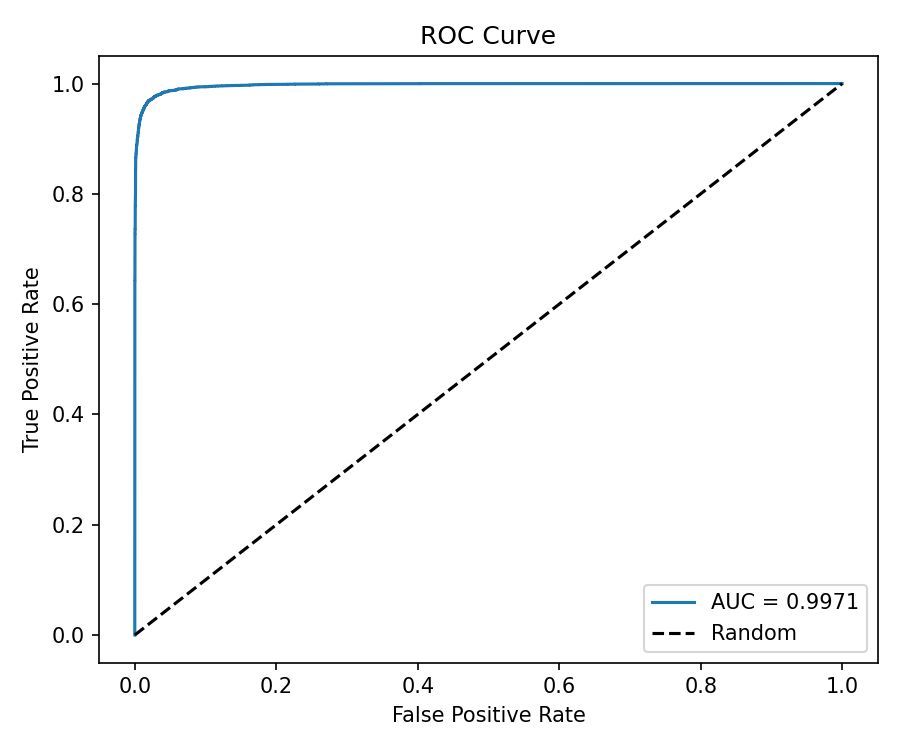
\includegraphics[width=0.7\textwidth]{../outputs/plots/roc_curve.png}
\caption{ROC curve (AUC = 0.9971).}
\label{fig:roc}
\end{figure}

\subsection{Train/Validation/Test Balance Verification}
\label{sec:balance}

The dataset splits were verified to be balanced (Table~\ref{tab:splits}). All splits contain approximately 50\% FAKE and 50\% REAL images. The identical preprocessing pipeline is applied to both classes via \texttt{ImageFolder} (see Section~5.4). There is no class imbalance that could explain differential performance.

\subsection{Addressing the Apparent Per-Class Performance Gap}

An earlier observation noted that two FAKE images in the Grad-CAM analysis had \textbf{confidence scores} of 70--72\%, while REAL images consistently showed 99--100\% confidence. It is important to clarify that \textbf{these are per-sample confidence scores on individual images, not per-class accuracy or recall}.

On the full 20,000-image test set, per-class performance is balanced:
\begin{itemize}[noitemsep]
    \item FAKE recall: 95.29\% (9,529 / 10,000 correctly detected)
    \item REAL recall: 98.63\% (9,863 / 10,000 correctly detected)
    \item FAKE precision: 98.58\%
    \item REAL precision: 95.44\%
\end{itemize}

Both classes achieve ${\sim}$97\% F1-score. The 70--72\% values refer to how confident the model was on two specific FAKE samples that it still classified \emph{correctly}. The lower confidence on those particular images indicates the model found them harder to distinguish --- a sign of good calibration rather than a systematic class imbalance. The confusion matrix (Table~\ref{tab:confusion}), precision/recall/F1 table (Table~\ref{tab:perclass}), ROC curve (Figure~\ref{fig:roc}), probability histograms (Figure~\ref{fig:probhist}), and split balance (Table~\ref{tab:splits}) all confirm there is no systematic bias favouring one class.

\subsection{Predicted Probability Distributions}

Histograms of $P(\text{FAKE})$ for actual FAKE and actual REAL images show well-separated distributions (Table~\ref{tab:probdist}, Figure~\ref{fig:probhist}).

\begin{table}[H]
\centering
\caption{Predicted probability statistics by true class.}
\label{tab:probdist}
\begin{tabular}{lcc}
\toprule
\textbf{True Class} & \textbf{Mean $P$(FAKE)} & \textbf{Median $P$(FAKE)} \\
\midrule
Actual FAKE & 0.9293 & 0.9983 \\
Actual REAL & 0.0244 & 0.0000 \\
\bottomrule
\end{tabular}
\end{table}

\begin{figure}[H]
\centering
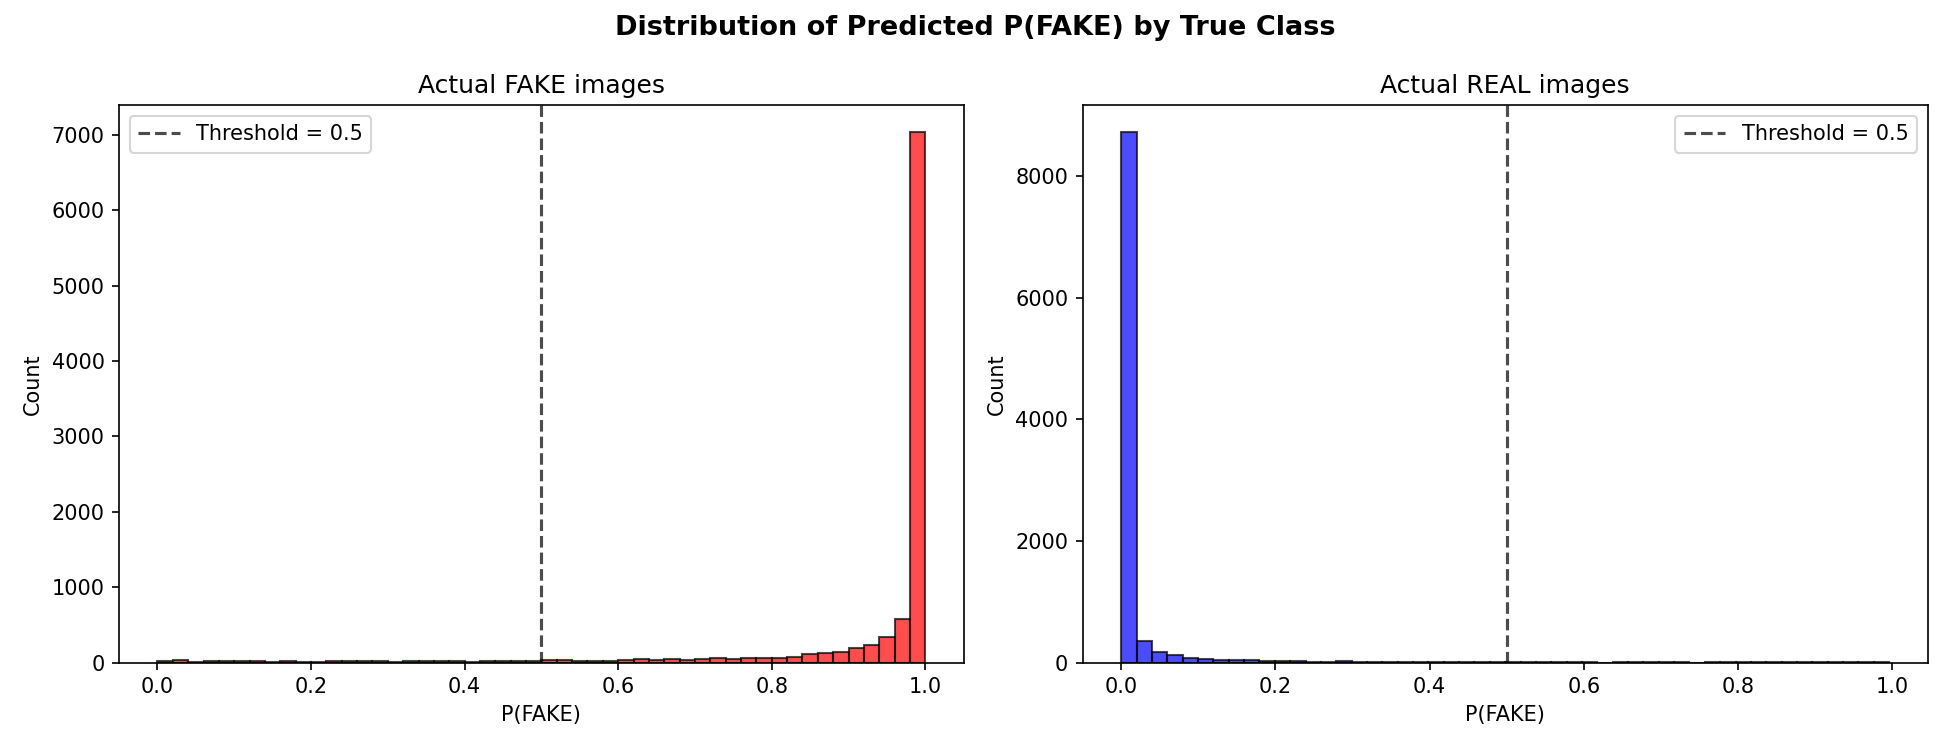
\includegraphics[width=0.75\textwidth]{../outputs/plots/probability_histograms.png}
\caption{Predicted probability distributions for FAKE and REAL images.}
\label{fig:probhist}
\end{figure}

\subsection{Threshold Sensitivity Analysis}

Varying the classification threshold from 0.40 to 0.70 (Table~\ref{tab:threshold}), all metrics remain above 91\%, demonstrating model robustness. The highest accuracy (97.22\%) occurs at threshold 0.40. As threshold increases, precision rises but recall drops --- the standard precision--recall trade-off.

Despite threshold 0.40 yielding the highest accuracy, the default of 0.50 is retained because the gap is marginal (97.22\% vs.\ 96.96\%, only 0.26\%).
A lower threshold increases false positives: precision drops from 0.9858 at 0.50 to 0.9635 at 0.40, meaning more real images are incorrectly flagged as AI-generated.
The 0.50 boundary represents the natural decision point where the model is more confident than not, making it more interpretable.
It is also more robust to shifts in class distribution at deployment time, where the real-to-fake ratio may differ from the balanced test set.
For applications that prioritise catching every AI image (e.g., content moderation), a lower threshold could be justified, but for a general-purpose detector the balanced default is preferable.

\begin{table}[H]
\centering
\caption{Threshold sensitivity analysis.}
\label{tab:threshold}
\begin{tabular}{ccccc}
\toprule
\textbf{Threshold} & \textbf{Accuracy} & \textbf{Precision} & \textbf{Recall} & \textbf{F1} \\
\midrule
0.40          & 0.9722 & 0.9807 & 0.9635 & 0.9720 \\
0.45          & 0.9716 & 0.9839 & 0.9589 & 0.9712 \\
\textbf{0.50} & \textbf{0.9696} & \textbf{0.9858} & \textbf{0.9529} & \textbf{0.9691} \\
0.55          & 0.9665 & 0.9871 & 0.9454 & 0.9658 \\
0.60          & 0.9646 & 0.9894 & 0.9393 & 0.9637 \\
0.65          & 0.9605 & 0.9906 & 0.9297 & 0.9592 \\
0.70          & 0.9563 & 0.9922 & 0.9197 & 0.9546 \\
\bottomrule
\end{tabular}
\end{table}

\begin{figure}[H]
\centering
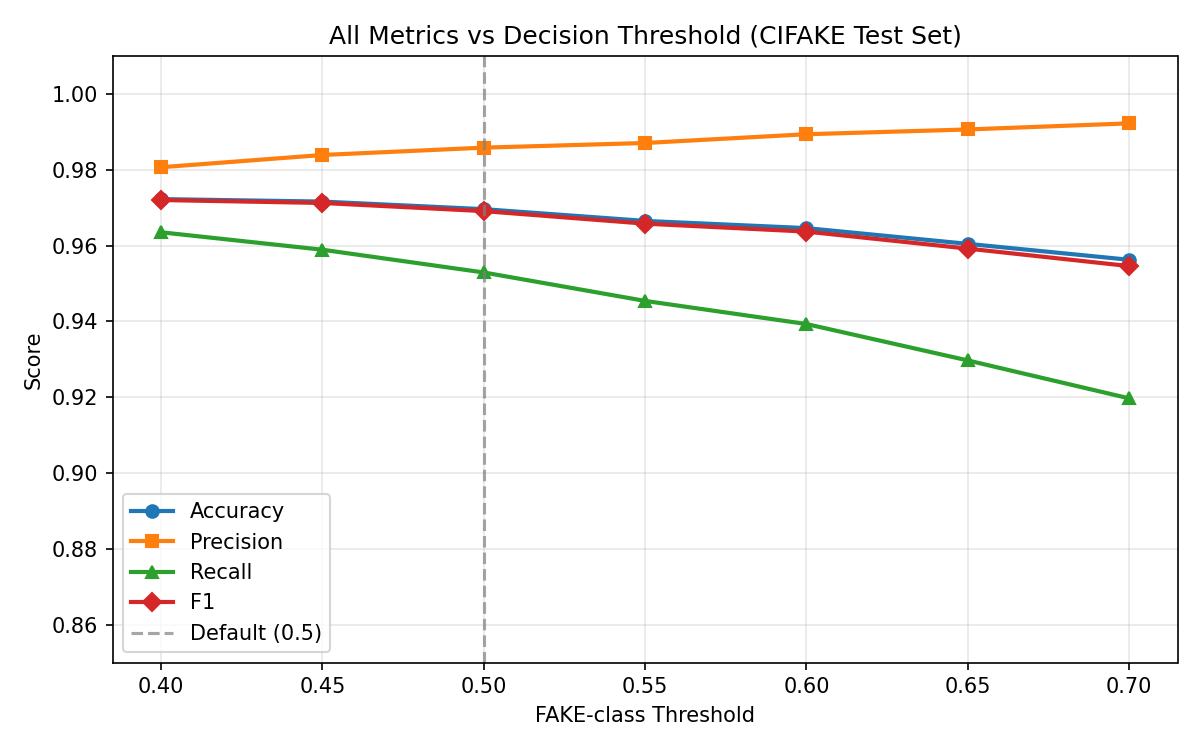
\includegraphics[width=0.75\textwidth]{../outputs/plots/threshold_all_metrics.png}
\caption{Threshold sensitivity --- all metrics.}
\label{fig:threshold_all}
\end{figure}

\begin{figure}[H]
\centering
\begin{subfigure}[b]{0.48\textwidth}
    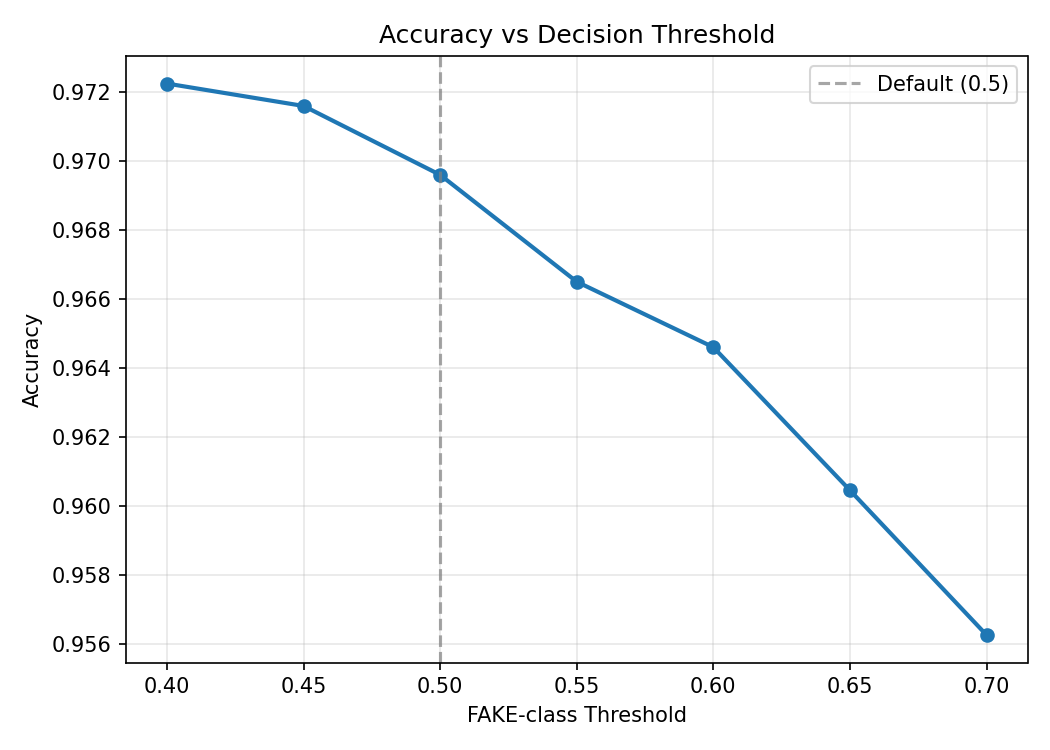
\includegraphics[width=\textwidth]{../outputs/plots/threshold_accuracy.png}
    \caption{Accuracy vs.\ threshold.}
\end{subfigure}
\hfill
\begin{subfigure}[b]{0.48\textwidth}
    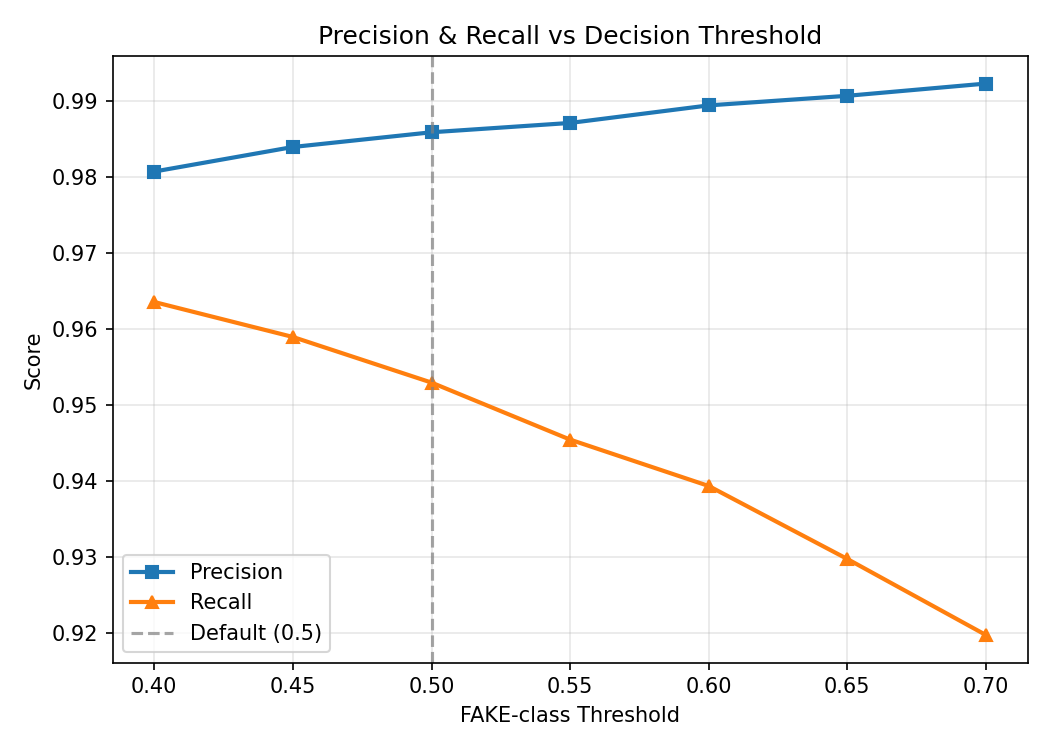
\includegraphics[width=\textwidth]{../outputs/plots/threshold_precision_recall.png}
    \caption{Precision/recall vs.\ threshold.}
\end{subfigure}
\caption{Threshold sensitivity breakdown.}
\label{fig:threshold_detail}
\end{figure}

\subsection{Temperature Scaling and Calibration}

The temperature parameter $T$ is \emph{learned} from the validation set via L-BFGS optimisation of negative log-likelihood. Table~\ref{tab:calibration} shows the results.

\begin{table}[H]
\centering
\caption{Calibration results (ECE = Expected Calibration Error).}
\label{tab:calibration}
\begin{tabular}{lccc}
\toprule
\textbf{Set} & \textbf{ECE Before} & \textbf{ECE After} & \textbf{Temperature} \\
\midrule
Validation (used to learn $T$) & 0.0031 & 0.0116 & 1.2189 \\
Test (held-out)                & 0.0026 & 0.0113 & 1.2189 \\
\bottomrule
\end{tabular}
\end{table}

The model was already very well-calibrated before temperature scaling (test ECE = 0.0026). Applying temperature scaling \emph{increased} ECE on both sets, meaning the single-parameter adjustment over-corrected an already well-calibrated model. Temperature scaling optimises negative log-likelihood, not ECE directly.

\begin{figure}[H]
\centering
\begin{subfigure}[b]{0.48\textwidth}
    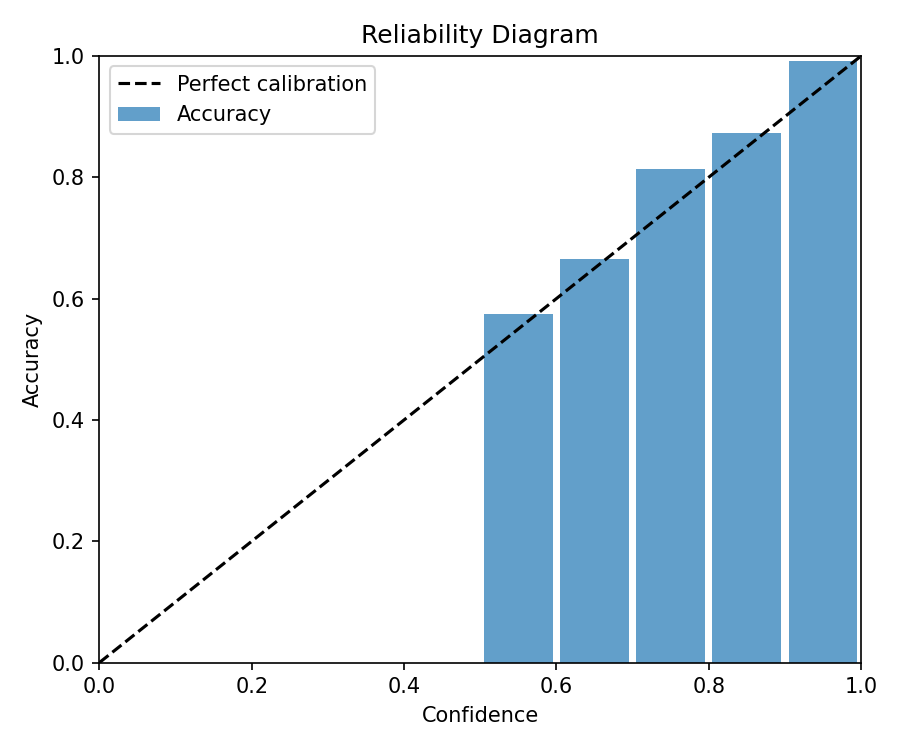
\includegraphics[width=\textwidth]{../outputs/plots/reliability_pre_calibration.png}
    \caption{Before calibration (ECE = 0.0026).}
\end{subfigure}
\hfill
\begin{subfigure}[b]{0.48\textwidth}
    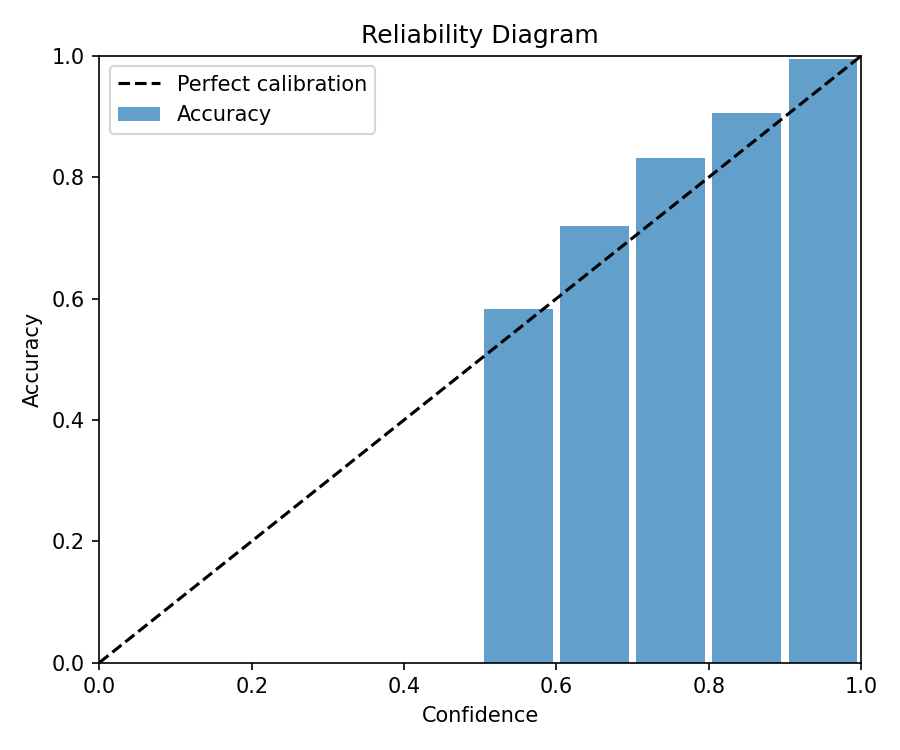
\includegraphics[width=\textwidth]{../outputs/plots/reliability_post_calibration.png}
    \caption{After calibration (ECE = 0.0113).}
\end{subfigure}
\caption{Reliability diagrams before and after temperature scaling.}
\label{fig:reliability}
\end{figure}

\begin{figure}[H]
\centering
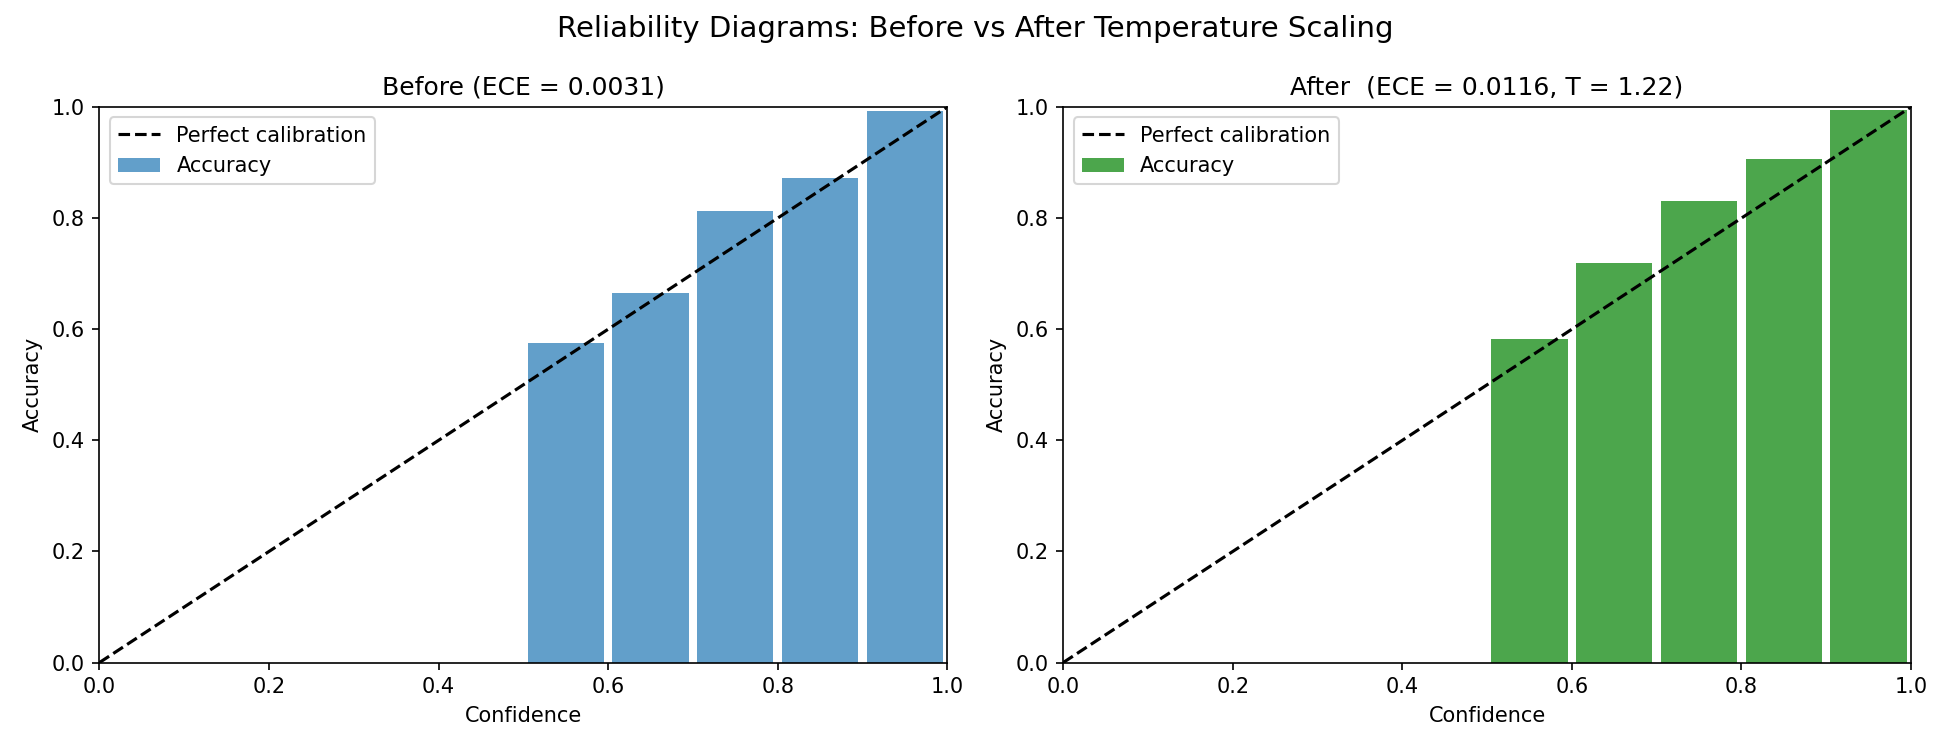
\includegraphics[width=0.75\textwidth]{../outputs/plots/calibration_comparison.png}
\caption{Calibration comparison (before vs.\ after temperature scaling).}
\label{fig:calibration_comparison}
\end{figure}

% ══════════════════════════════════════════════════════════════
\section{Analysis and Discussion}

\subsection{Misclassified FAKE Images: Do They Appear Realistic?}

471 FAKE images were misclassified as REAL out of 10,000 (4.71\% false-negative rate). Figure~\ref{fig:misclassified} shows the most confidently misclassified samples (highest $P(\text{REAL})$).

\textbf{Visual inspection findings:} The misclassified FAKE images do appear notably more realistic than typical CIFAKE fakes. Specifically:
\begin{itemize}[noitemsep]
    \item \textbf{Fewer visible generation artefacts:} These images lack the subtle over-smoothing, colour banding, and texture repetition commonly seen in Stable Diffusion v1.4 outputs. Their textures appear more natural and varied.
    \item \textbf{More realistic compositions:} The spatial layout, object placement, and colour distributions closely resemble natural photographs from CIFAR-10. There are no obvious structural inconsistencies (e.g., distorted edges, unnatural symmetry).
    \item \textbf{Natural colour distributions:} Unlike many CIFAKE fakes that exhibit slightly saturated or uniform colour palettes, these misclassified images have colour statistics closer to the real image distribution.
\end{itemize}

\textbf{Why does the model fail on these?} The model primarily relies on low-level texture artefacts specific to Stable Diffusion v1.4 (as confirmed by Grad-CAM analysis in Section~\ref{sec:gradcam}). When a generated image happens to have fewer of these artefacts --- either due to the specific prompt, random seed, or content type --- the model lacks sufficient signal to distinguish it from a real image. These images sit closest to the decision boundary in probability space ($P(\text{FAKE})$ near 0.5 rather than near 1.0).

This finding is consistent with Gragnaniello et al.\ (2021), who showed that some generated images fall closer to the decision boundary in feature space due to reduced generator-specific fingerprints. It also reinforces the project's central hypothesis: if even \emph{within} the training distribution some images evade detection by lacking artefacts, images from \emph{newer} generators that systematically produce fewer artefacts will be even harder to detect.

\begin{figure}[H]
\centering
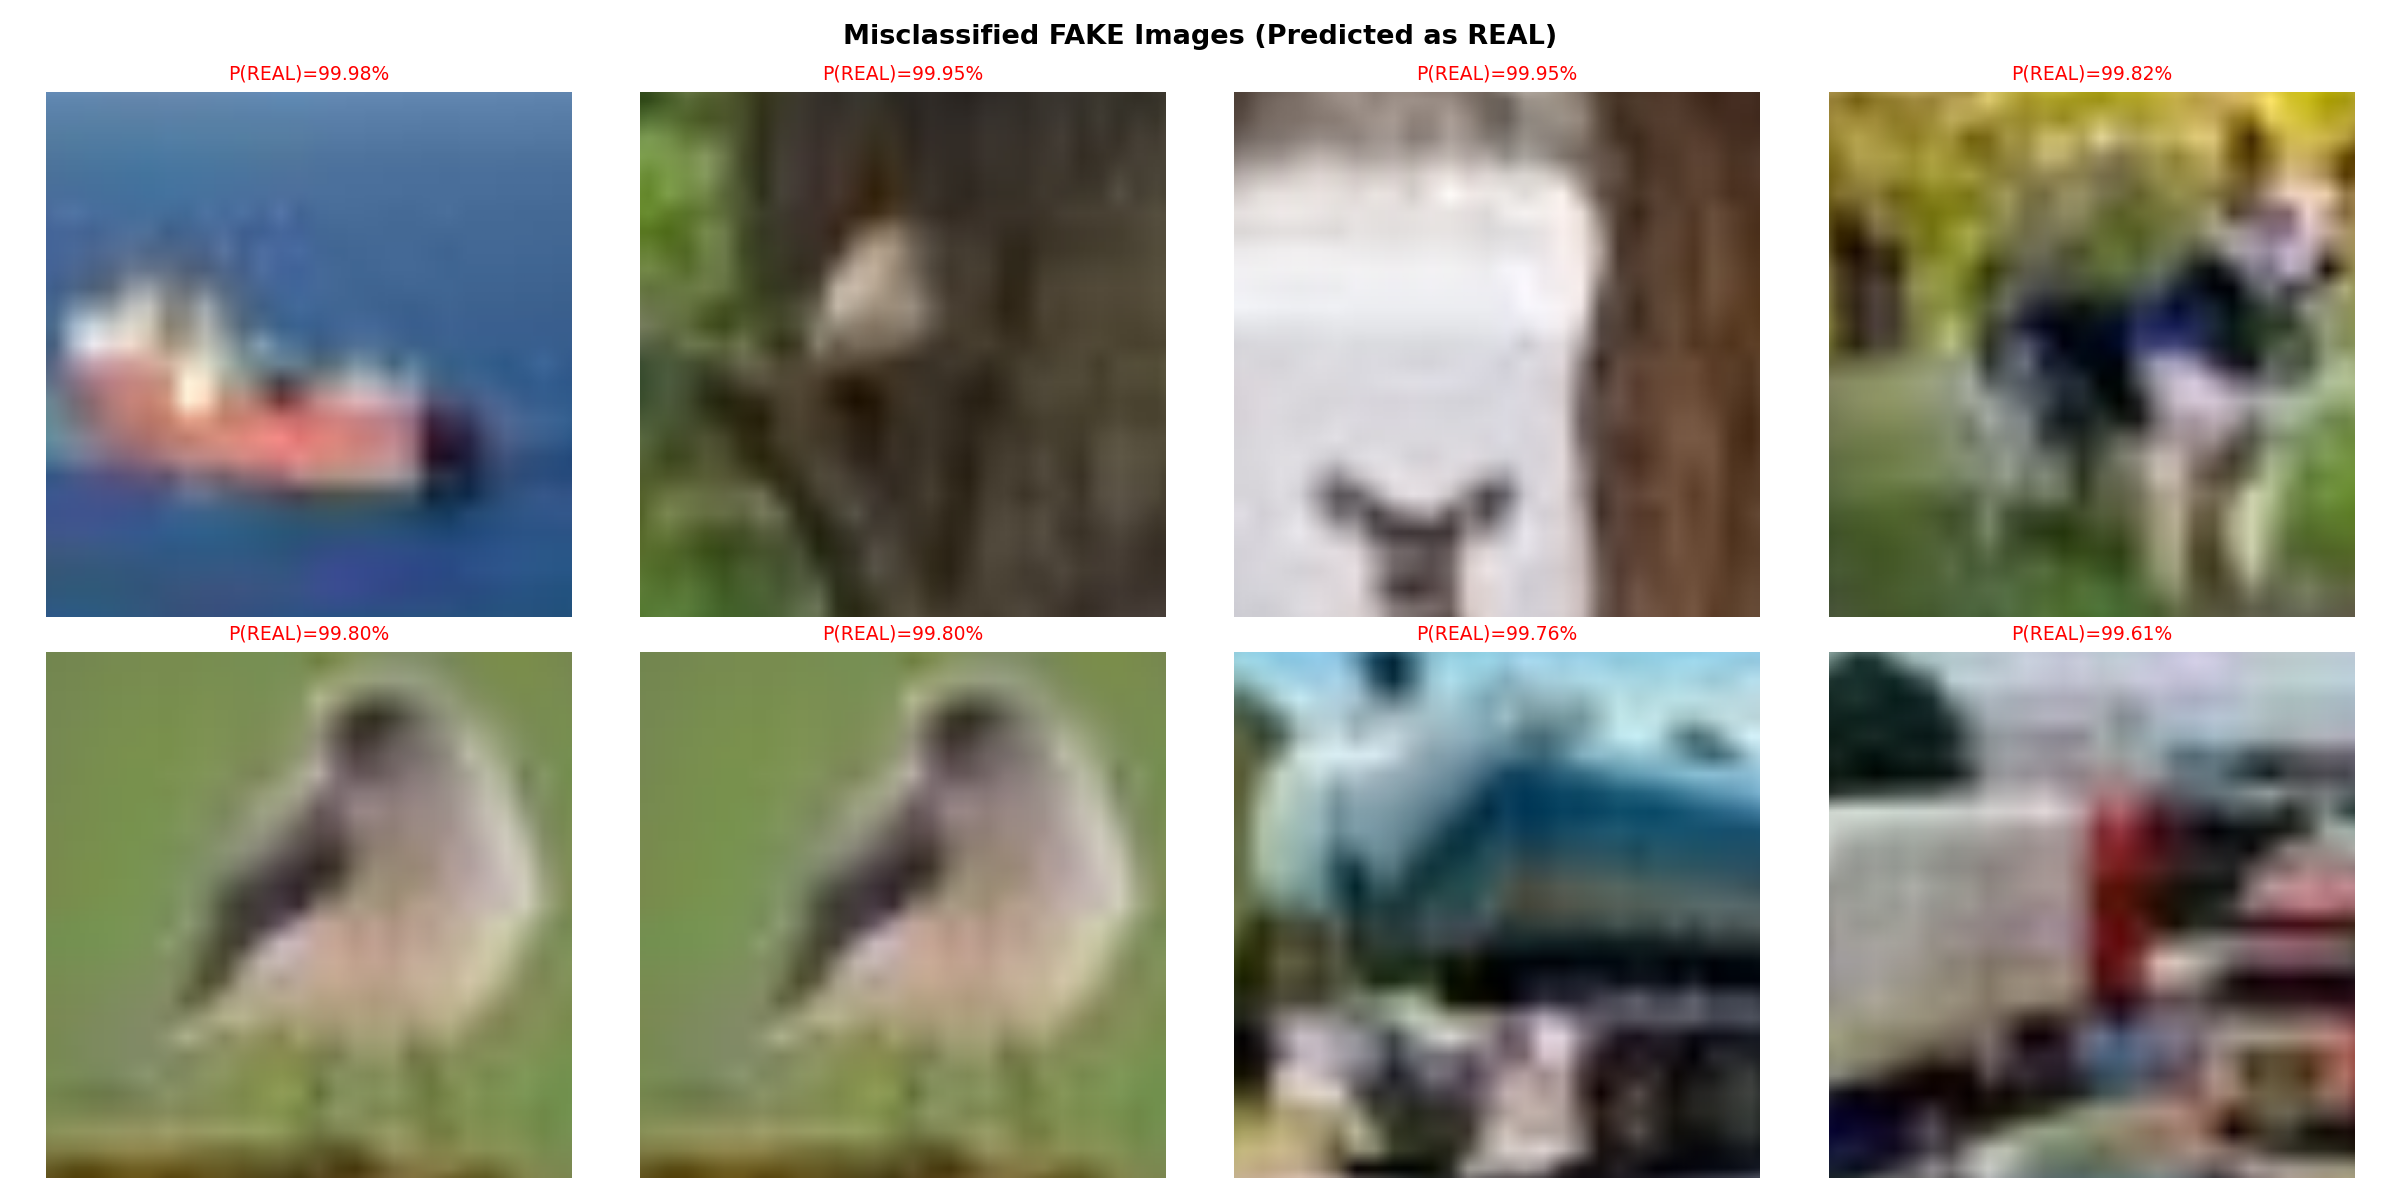
\includegraphics[width=0.85\textwidth]{../outputs/plots/misclassified_fakes.png}
\caption{Most confidently misclassified FAKE images (predicted as REAL).}
\label{fig:misclassified}
\end{figure}

\subsection{Grad-CAM Findings}
\label{sec:gradcam}

Grad-CAM heatmaps reveal systematic differences in the model's attention:

\begin{itemize}[noitemsep]
    \item \textbf{REAL images:} Broad, diffuse attention across the image, focusing on fine-grained texture regions. Confidence uniformly high (99--100\%).
    \item \textbf{FAKE images:} More localised attention patterns. High-confidence predictions focus on regions with visible generation artefacts. Lower-confidence predictions (70--72\%) show more scattered activation, suggesting the model is uncertain about which regions contain artefacts.
\end{itemize}

This indicates the model primarily relies on \textbf{low-level texture artefacts specific to Stable Diffusion v1.4}. This finding directly supports the project's hypothesis: the detector has learned distribution-specific features that may not transfer to newer generators.

\begin{figure}[H]
\centering
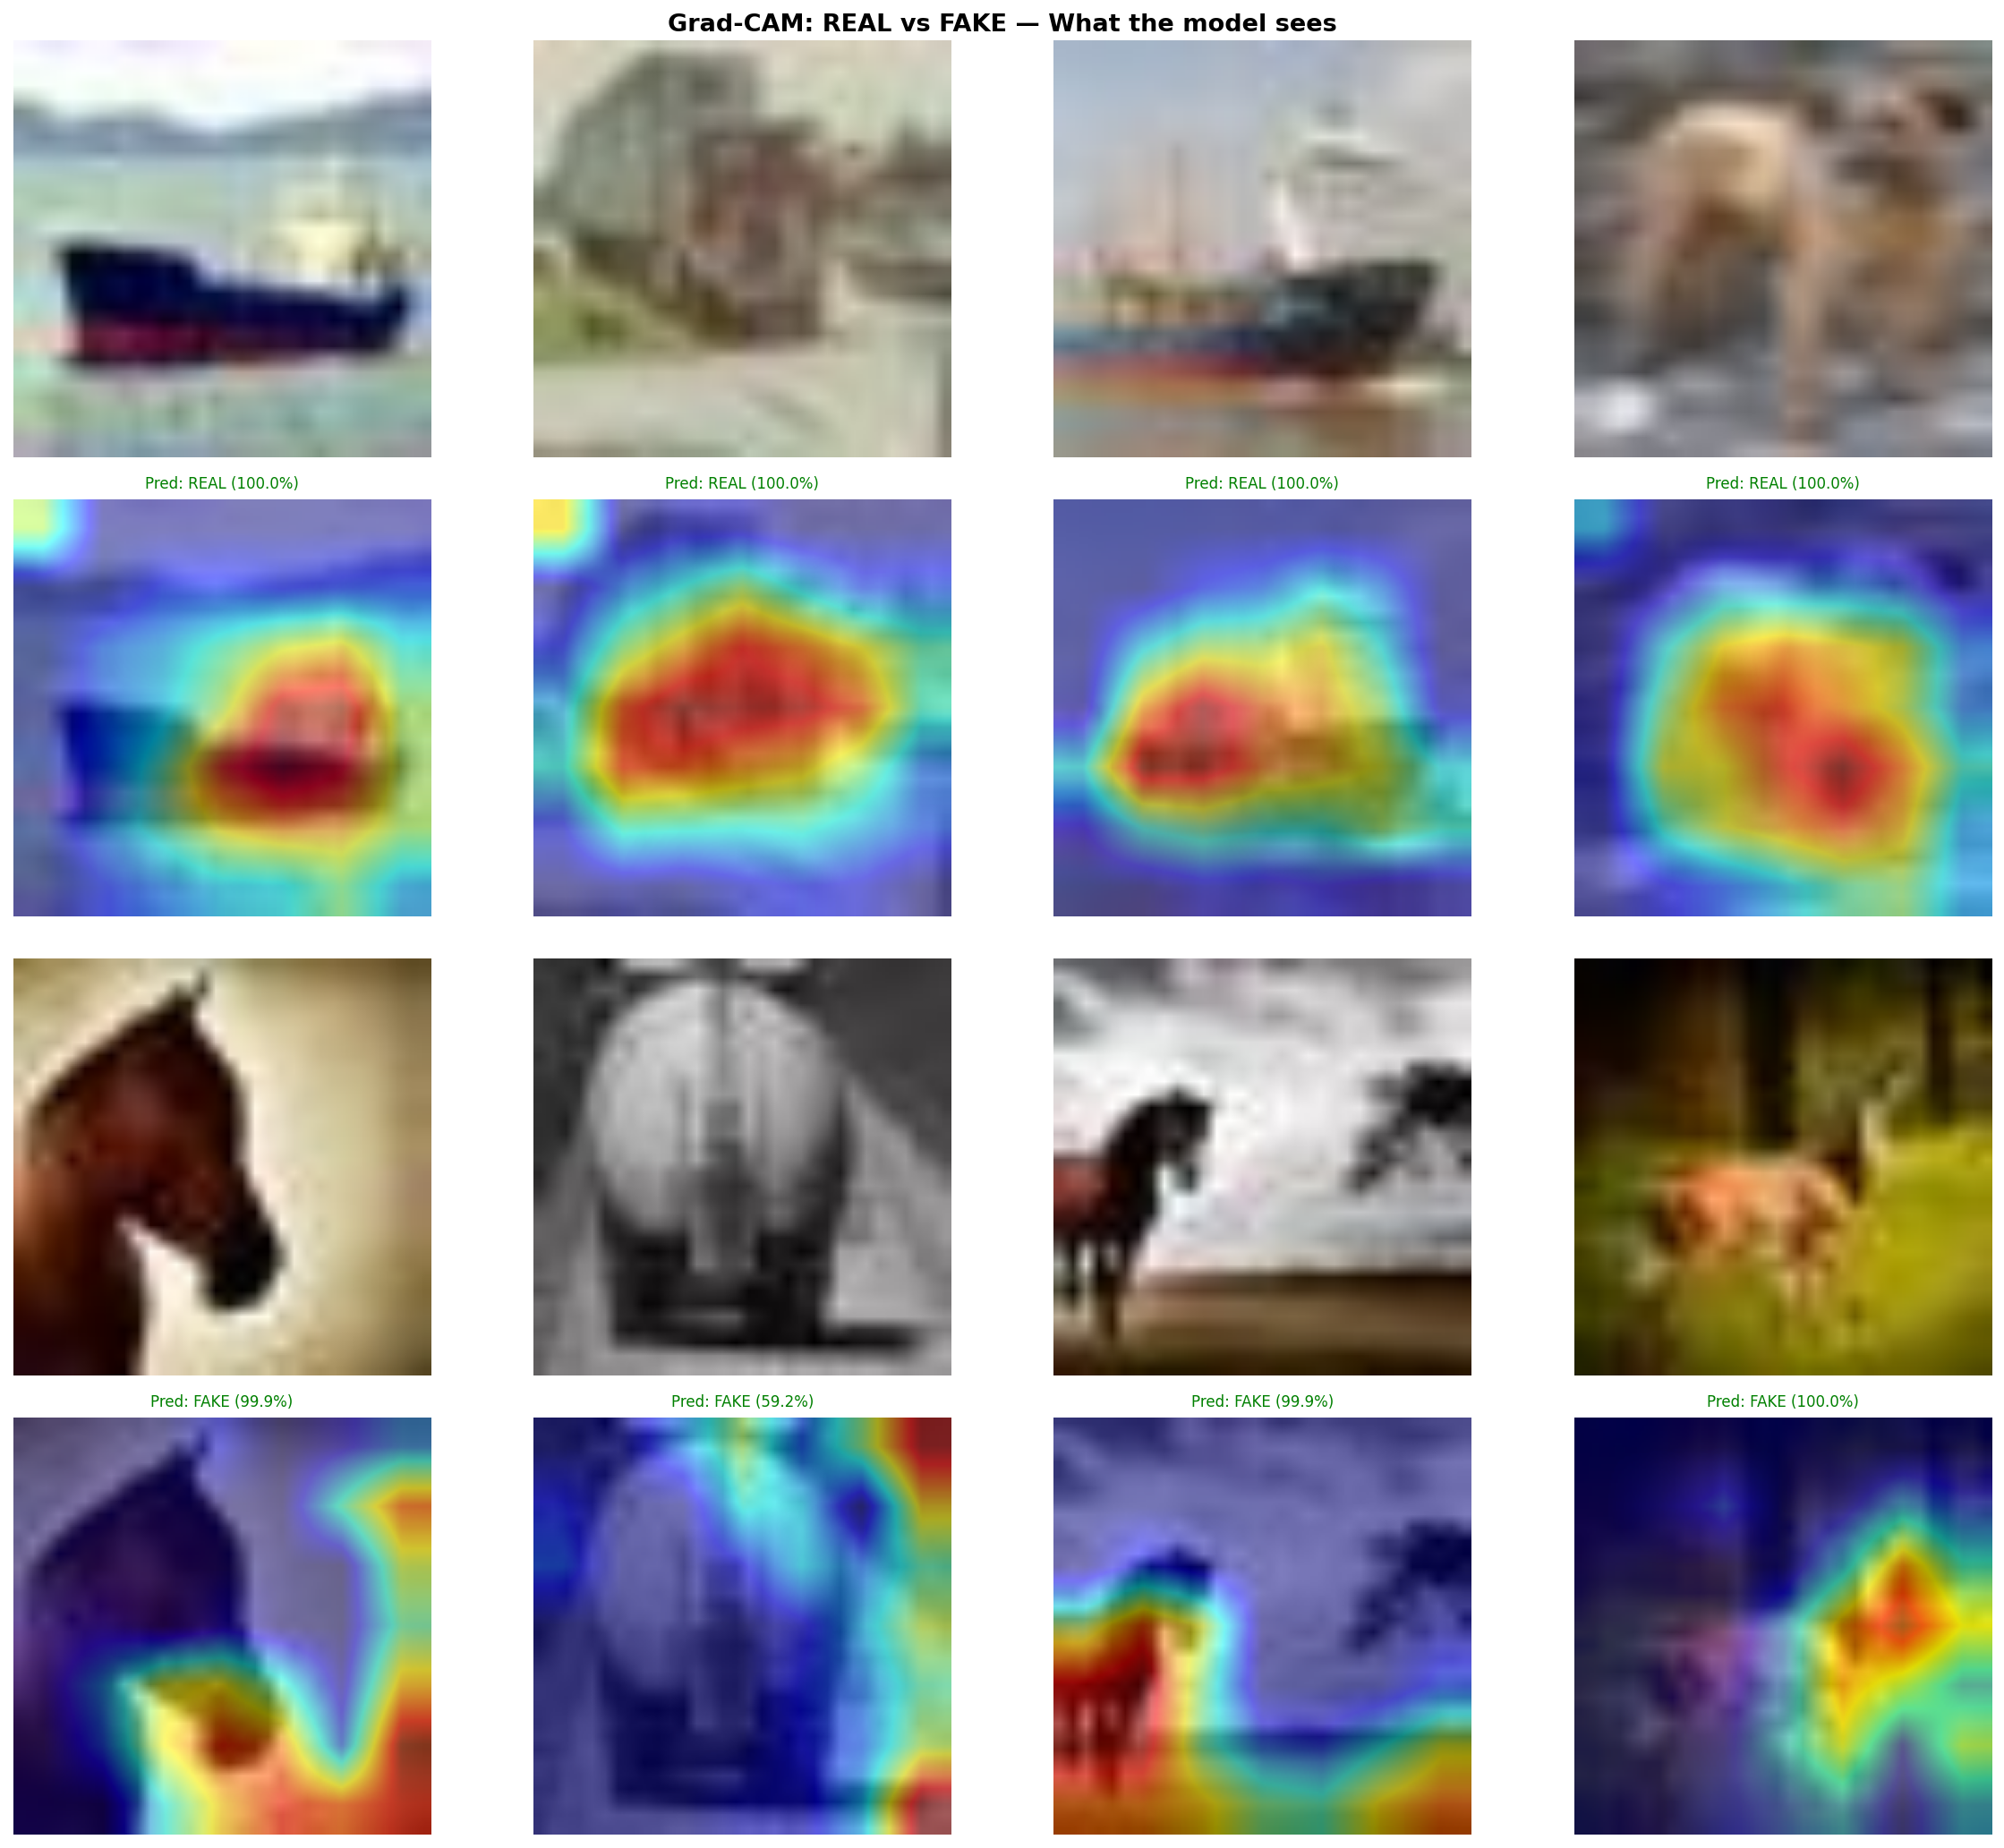
\includegraphics[width=0.95\textwidth]{../outputs/plots/gradcam_comparison.png}
\caption{Grad-CAM comparison --- FAKE vs.\ REAL images.}
\label{fig:gradcam_comparison}
\end{figure}

\begin{figure}[H]
\centering
\begin{subfigure}[b]{0.48\textwidth}
    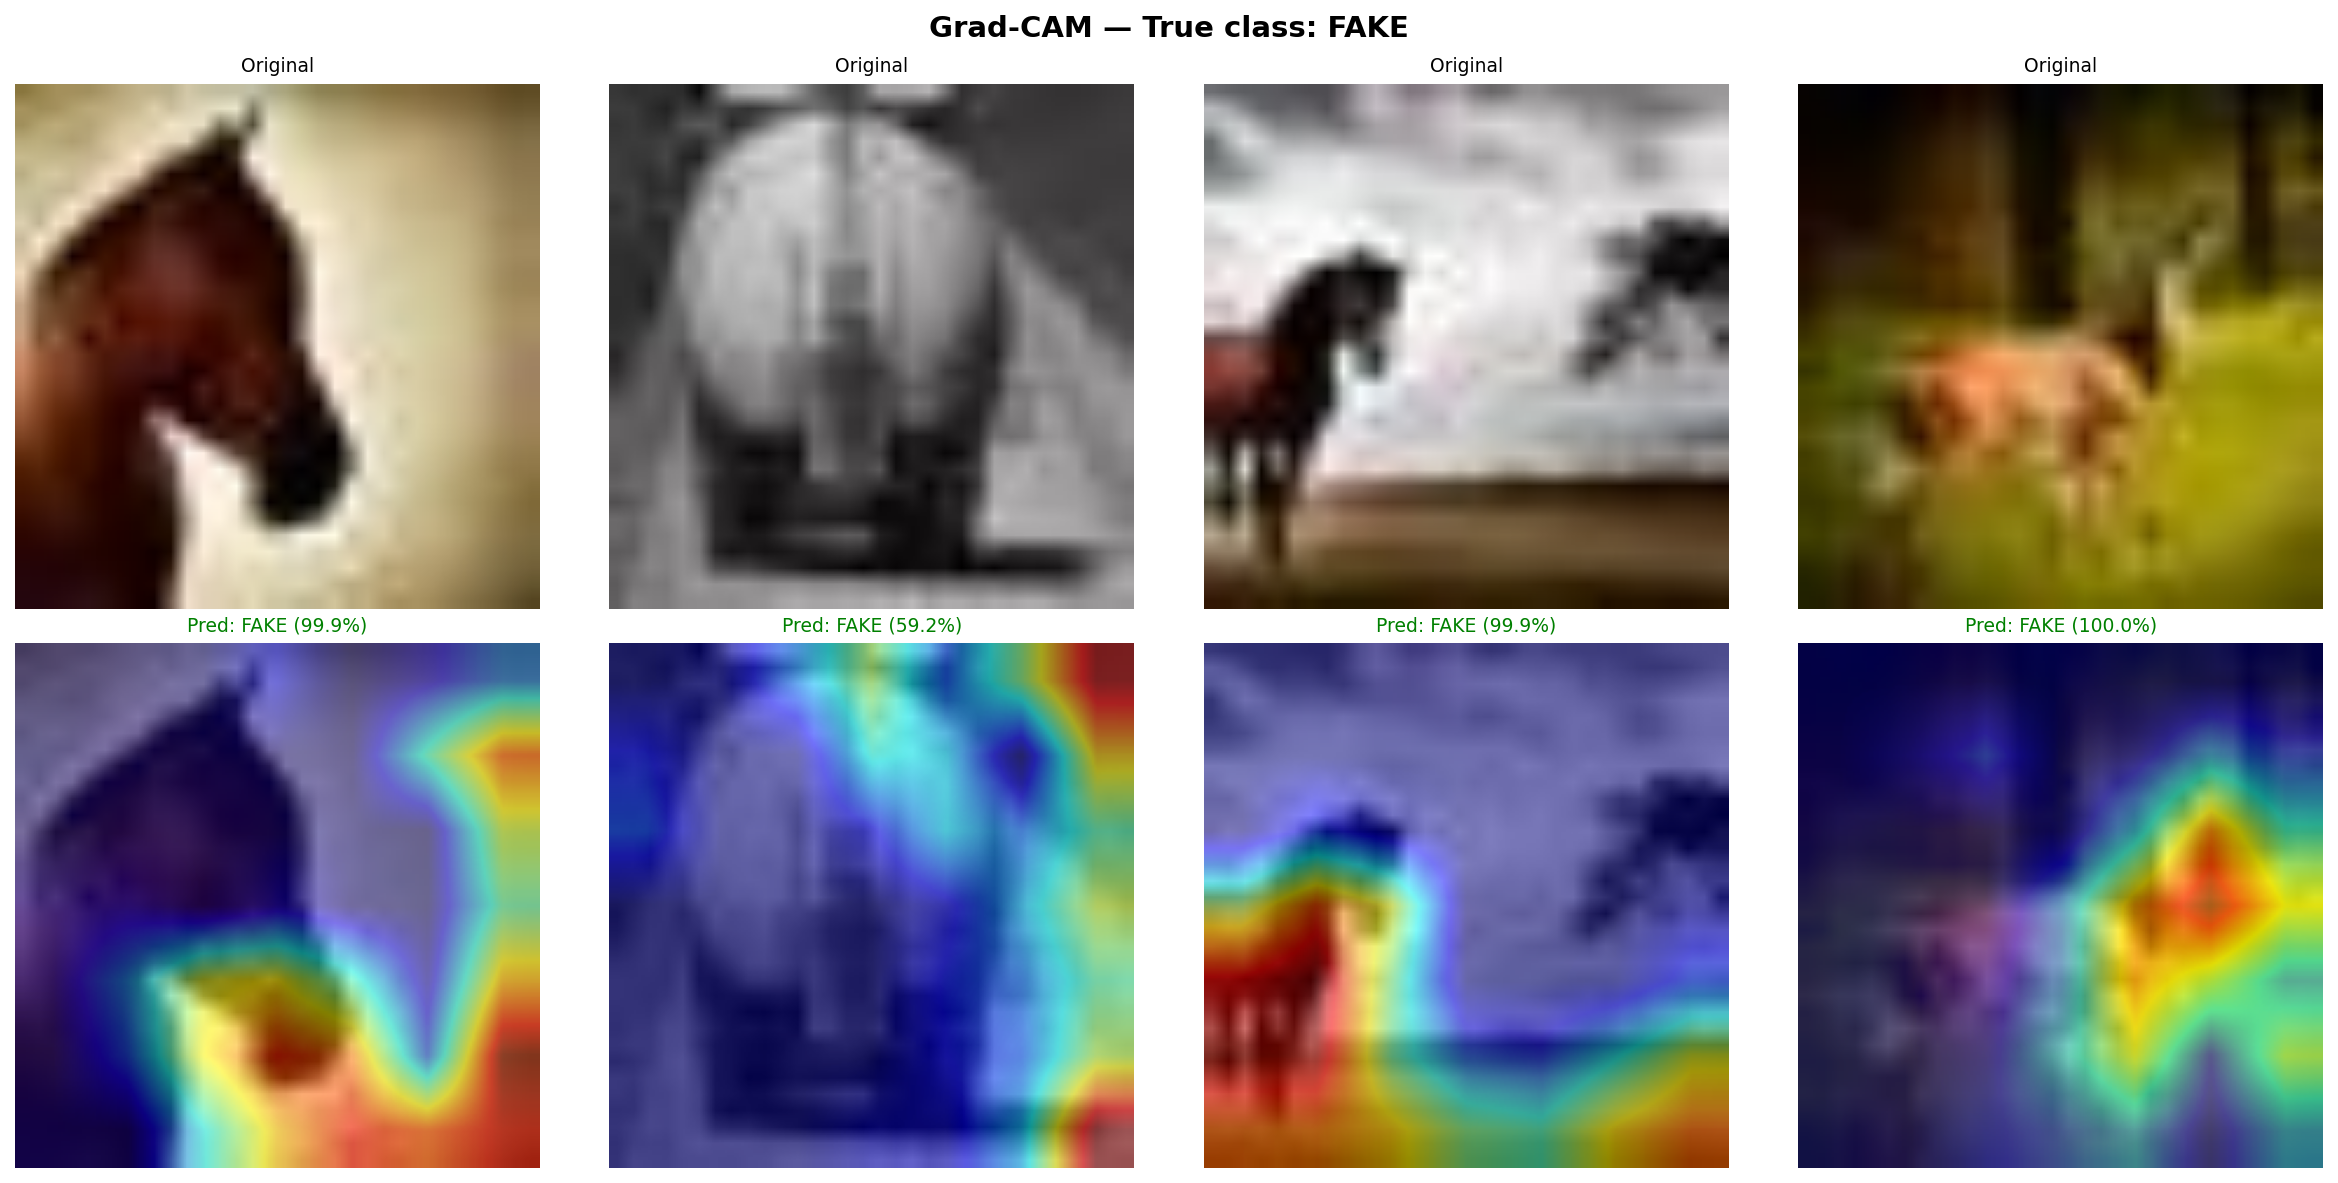
\includegraphics[width=\textwidth]{../outputs/plots/gradcam_fake.png}
    \caption{Grad-CAM on FAKE images.}
\end{subfigure}
\hfill
\begin{subfigure}[b]{0.48\textwidth}
    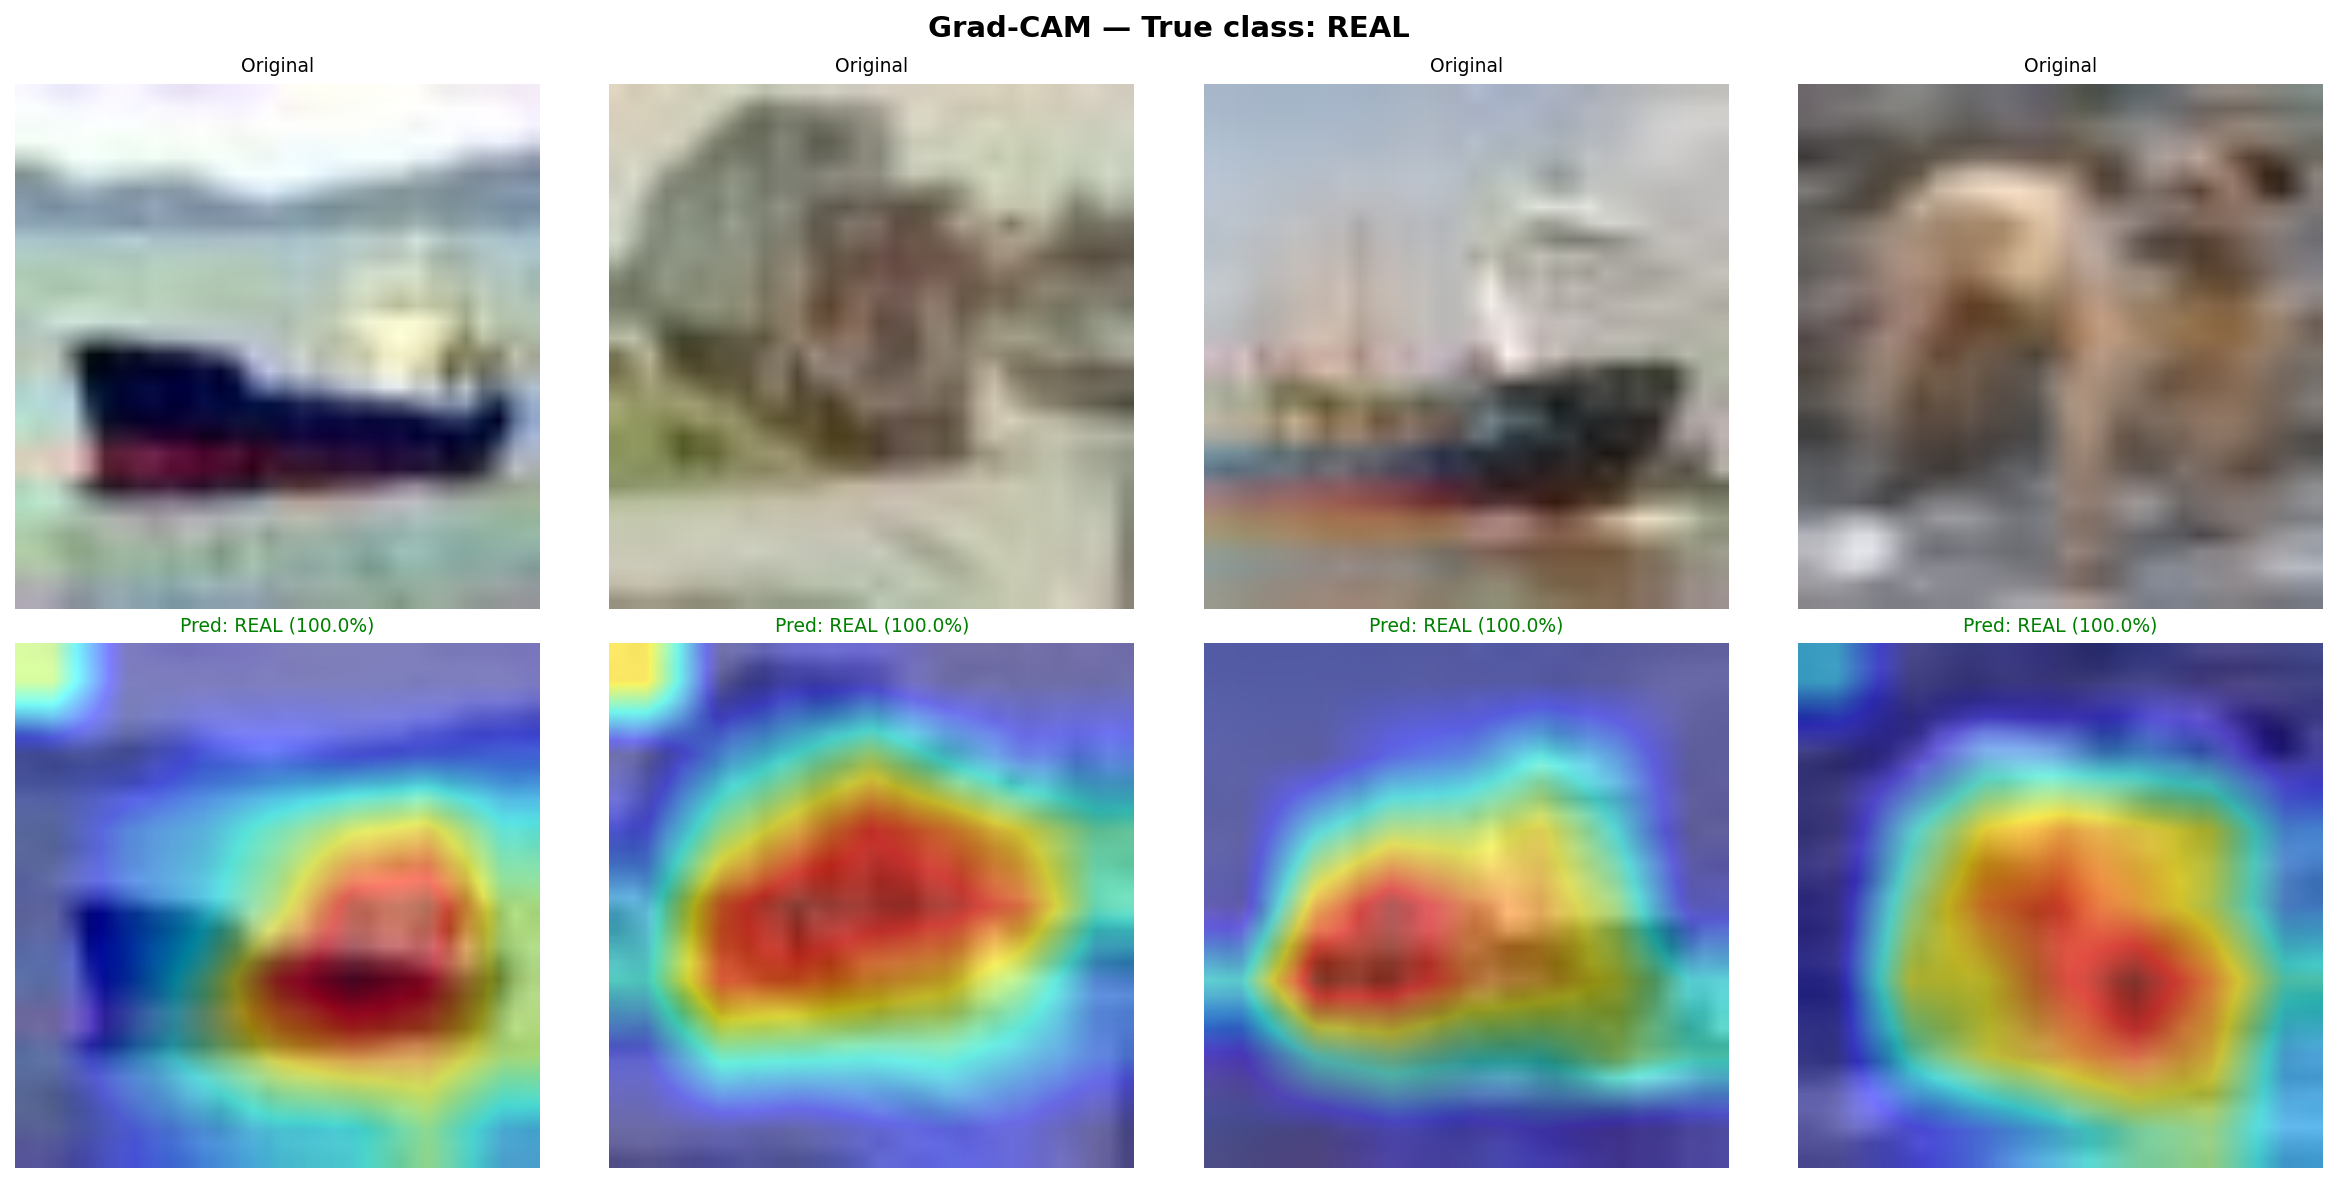
\includegraphics[width=\textwidth]{../outputs/plots/gradcam_real.png}
    \caption{Grad-CAM on REAL images.}
\end{subfigure}
\caption{Grad-CAM heatmaps by class.}
\label{fig:gradcam_classes}
\end{figure}

\subsubsection{Individual Grad-CAM Heatmaps}

Figures~\ref{fig:heatmaps_fake} and~\ref{fig:heatmaps_real} show individual Grad-CAM heatmaps for selected FAKE and REAL test samples. FAKE images exhibit localised ``hotspots'' where the model detects generation artefacts, while REAL images show diffuse attention spread across natural textures.

\begin{figure}[H]
\centering
\begin{subfigure}[b]{0.24\textwidth}
    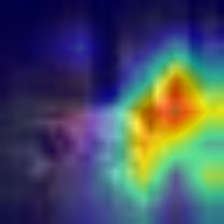
\includegraphics[width=\textwidth]{../outputs/heatmaps/FAKE_48 (5).jpg}
\end{subfigure}
\begin{subfigure}[b]{0.24\textwidth}
    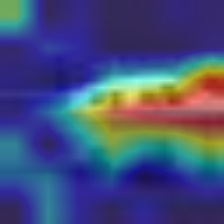
\includegraphics[width=\textwidth]{../outputs/heatmaps/FAKE_516.jpg}
\end{subfigure}
\begin{subfigure}[b]{0.24\textwidth}
    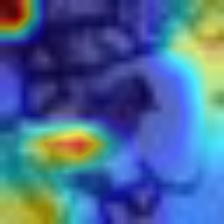
\includegraphics[width=\textwidth]{../outputs/heatmaps/FAKE_518 (3).jpg}
\end{subfigure}
\begin{subfigure}[b]{0.24\textwidth}
    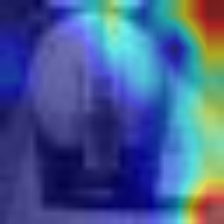
\includegraphics[width=\textwidth]{../outputs/heatmaps/FAKE_52 (10).jpg}
\end{subfigure}

\begin{subfigure}[b]{0.24\textwidth}
    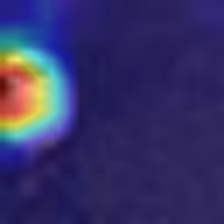
\includegraphics[width=\textwidth]{../outputs/heatmaps/FAKE_636 (3).jpg}
\end{subfigure}
\begin{subfigure}[b]{0.24\textwidth}
    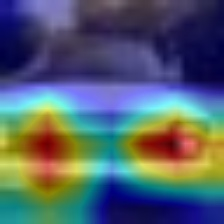
\includegraphics[width=\textwidth]{../outputs/heatmaps/FAKE_755 (2).jpg}
\end{subfigure}
\begin{subfigure}[b]{0.24\textwidth}
    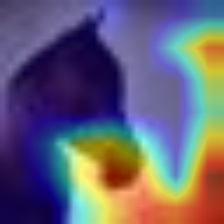
\includegraphics[width=\textwidth]{../outputs/heatmaps/FAKE_870 (8).jpg}
\end{subfigure}
\begin{subfigure}[b]{0.24\textwidth}
    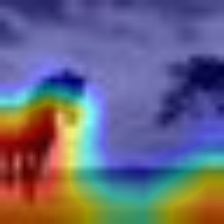
\includegraphics[width=\textwidth]{../outputs/heatmaps/FAKE_95 (8).jpg}
\end{subfigure}
\caption{Individual Grad-CAM heatmaps for FAKE images --- localised attention on generation artefacts.}
\label{fig:heatmaps_fake}
\end{figure}

\begin{figure}[H]
\centering
\begin{subfigure}[b]{0.24\textwidth}
    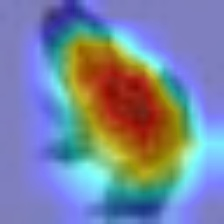
\includegraphics[width=\textwidth]{../outputs/heatmaps/REAL_0066 (7).jpg}
\end{subfigure}
\begin{subfigure}[b]{0.24\textwidth}
    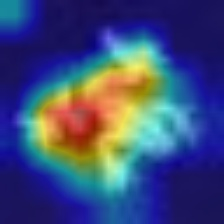
\includegraphics[width=\textwidth]{../outputs/heatmaps/REAL_0090 (7).jpg}
\end{subfigure}
\begin{subfigure}[b]{0.24\textwidth}
    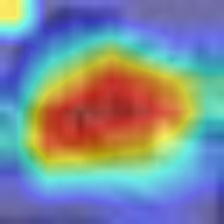
\includegraphics[width=\textwidth]{../outputs/heatmaps/REAL_0124 (10).jpg}
\end{subfigure}
\begin{subfigure}[b]{0.24\textwidth}
    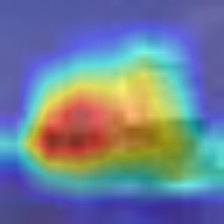
\includegraphics[width=\textwidth]{../outputs/heatmaps/REAL_0233 (9).jpg}
\end{subfigure}

\begin{subfigure}[b]{0.24\textwidth}
    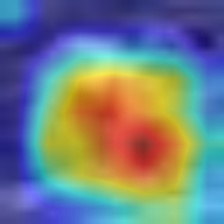
\includegraphics[width=\textwidth]{../outputs/heatmaps/REAL_0389 (6).jpg}
\end{subfigure}
\begin{subfigure}[b]{0.24\textwidth}
    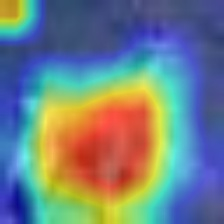
\includegraphics[width=\textwidth]{../outputs/heatmaps/REAL_0504 (5).jpg}
\end{subfigure}
\begin{subfigure}[b]{0.24\textwidth}
    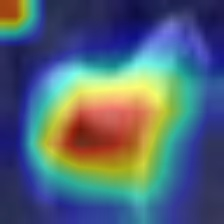
\includegraphics[width=\textwidth]{../outputs/heatmaps/REAL_0934 (8).jpg}
\end{subfigure}
\begin{subfigure}[b]{0.24\textwidth}
    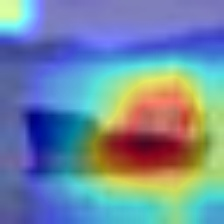
\includegraphics[width=\textwidth]{../outputs/heatmaps/REAL_0998 (9).jpg}
\end{subfigure}
\caption{Individual Grad-CAM heatmaps for REAL images --- diffuse attention across natural textures.}
\label{fig:heatmaps_real}
\end{figure}

\subsection{Calibration Discussion}

The model achieved an ECE of 0.0026 before calibration, which is remarkably low --- when the model says it is 95\% confident, it is correct approximately 95\% of the time. Temperature scaling learned $T = 1.2189$, confirming slight overconfidence as expected for modern deep networks (Guo et al., 2017). However, because the pre-calibration ECE was already so low, applying temperature scaling actually \emph{increased} ECE slightly to 0.0113. This is a known edge case with temperature scaling --- it optimises negative log-likelihood, not ECE directly, and on already well-calibrated models the correction can be counterproductive.

% ══════════════════════════════════════════════════════════════
\section{Completed Milestones}

\subsection{Milestone 1: Literature Review and Project Setup (Up to May 20)}

\begin{itemize}[noitemsep]
    \item Conducted literature review covering CNN-based detection methods (Wang et al., 2020; Bird \& Lotfi, 2024), generative model evolution (Corvi et al., 2023; Gragnaniello et al., 2021), explainability via Grad-CAM (Selvaraju et al., 2017), and calibration techniques (Guo et al., 2017).
    \item Identified research gap: no prior work combines cross-generator evaluation, calibration analysis, and Grad-CAM comparison across generator families.
    \item Set up GitHub repository and Google Colab environment.
    \item Downloaded and preprocessed CIFAKE dataset (60,000 images, balanced binary classification).
    \item Defined evaluation metrics: Accuracy, AUC-ROC, Expected Calibration Error (ECE).
    \item Prepared background summary and preliminary project specification.
\end{itemize}

\subsection{Milestone 2: Baseline Detector Development (May 21 -- June 15)}

\begin{itemize}[noitemsep]
    \item Developed baseline detector by fine-tuning EfficientNet-B3 (pretrained on ImageNet) on CIFAKE.
    \item Performed hyperparameter tuning via a 6-combination sweep (2 learning rates $\times$ 3 weight decays), selecting the best configuration based on validation accuracy.
    \item Achieved stable validation performance: 96.94\% validation accuracy at epoch 2.
    \item Implemented temperature scaling for confidence calibration, learning $T = 1.2189$ from the validation set via L-BFGS optimisation.
    \item Began initial evaluation: test accuracy 96.96\%, AUC-ROC 0.9971.
\end{itemize}

\subsection{Milestone 3: Explainability and Calibration Analysis (June 16 -- July 5)}

\begin{itemize}[noitemsep]
    \item Integrated Grad-CAM into the model pipeline, targeting the last convolutional block of EfficientNet-B3.
    \item Generated and analysed heatmaps for both FAKE and REAL images, revealing that the model attends to localised texture artefacts in FAKE images and diffuse natural textures in REAL images.
    \item Refined calibration analysis using Expected Calibration Error (ECE) and reliability diagrams, showing the model was already well-calibrated (ECE = 0.0026) before temperature scaling.
    \item Conducted threshold sensitivity analysis across 7 thresholds (0.40--0.70), confirming model robustness.
    \item Analysed misclassified FAKE images, identifying that failures correlate with reduced generation artefacts.
    \item Ensured evaluation pipeline is stable and reproducible (26 unit tests passing, fixed random seed 42).
\end{itemize}

% ══════════════════════════════════════════════════════════════
\section{Current Limitations and Planned Next Steps}

\subsection{Limitations}

\begin{enumerate}[noitemsep]
    \item \textbf{Single-generator training data.} The model is trained exclusively on CIFAKE, which contains images from Stable Diffusion v1.4. Its performance on images from other generators is unknown.
    \item \textbf{Low input resolution.} CIFAKE images are $32 \times 32$, which limits the amount of high-frequency detail available for detection. Higher-resolution datasets may reveal different artefact patterns.
    \item \textbf{Generator-specific features.} Grad-CAM analysis suggests the model relies on Stable Diffusion-specific texture artefacts, which newer generators may not produce.
\end{enumerate}

\subsection{Planned Next Steps}

\begin{table}[H]
\centering
\caption{Planned milestones.}
\label{tab:milestones}
\begin{tabular}{lll}
\toprule
\textbf{Milestone} & \textbf{Period} & \textbf{Tasks} \\
\midrule
4 --- Generalisation & Jul 6--20 & \parbox[t]{7.5cm}{Evaluate detector on StyleGAN, Stable Diffusion, Midjourney~v6, and GPT-4o images. Measure performance degradation. Analyse failure cases with Grad-CAM.} \\[1em]
5 --- Interactive Demo & Jul 21--Aug 10 & \parbox[t]{7.5cm}{Build Gradio web interface combining model, calibration, and Grad-CAM. End-to-end testing.} \\[1em]
6 --- Final Report & Aug 11--28 & \parbox[t]{7.5cm}{Write final report. Prepare visualisations. Finalise codebase and documentation.} \\
\bottomrule
\end{tabular}
\end{table}

% ══════════════════════════════════════════════════════════════
\section{Repository}

All code, notebooks, tests, and results are available at:\\
\url{https://github.com/krishi-shah/ai-image-detection}

\subsection*{Notebooks}
\begin{itemize}[noitemsep]
    \item \texttt{01\_setup\_and\_eda.ipynb} --- Environment setup, CIFAKE download and EDA
    \item \texttt{02\_baseline\_training.ipynb} --- Hyperparameter sweep and full training
    \item \texttt{03\_calibration.ipynb} --- Temperature scaling, threshold analysis, confusion matrix, ROC curve
    \item \texttt{04\_gradcam.ipynb} --- Grad-CAM heatmap generation and analysis
\end{itemize}

\subsection*{Source Modules}
\begin{itemize}[noitemsep]
    \item \texttt{src/model/detector.py} --- EfficientNet-B3 build, checkpoint save/load
    \item \texttt{src/evaluation/metrics.py} --- Accuracy, AUC, ECE, reliability diagrams, ROC curves
    \item \texttt{src/evaluation/calibration.py} --- Temperature scaling (learned via L-BFGS)
    \item \texttt{src/explainability/gradcam.py} --- Grad-CAM heatmap generation and overlay
    \item \texttt{src/utils/data\_loader.py} --- CIFAKE data loading with train/val/test splits
\end{itemize}

\subsection*{Tests}
26 unit tests across 5 test modules, all passing --- covering model architecture, data transforms, evaluation metrics, calibration, and Grad-CAM.

% ══════════════════════════════════════════════════════════════
\section*{References}

\begin{enumerate}[label={[\arabic*]}, noitemsep]
    \item Bird, J.J.\ \& Lotfi, A.\ (2024). CIFAKE: Image Classification and Explainable Identification of AI-Generated Synthetic Images. \textit{IEEE Access}, 12, 15642--15650.
    \item Corvi, R.\ et al.\ (2023). On the Detection of Synthetic Images Generated by Diffusion Models. \textit{ICASSP 2023}.
    \item Gragnaniello, D.\ et al.\ (2021). Are GAN Generated Images Easy to Detect? A Critical Analysis of the State of the Art. \textit{ICME 2021}.
    \item Guo, C.\ et al.\ (2017). On Calibration of Modern Neural Networks. \textit{ICML 2017}.
    \item Selvaraju, R.\ et al.\ (2017). Grad-CAM: Visual Explanations from Deep Networks via Gradient-based Localization. \textit{ICCV 2017}.
    \item Wang, S.\ et al.\ (2020). CNN-Generated Images Are Surprisingly Easy to Spot\ldots For Now. \textit{CVPR 2020}.
\end{enumerate}

\end{document}
